\documentclass[runningheads]{llncs}
\usepackage[T1]{fontenc}
\usepackage{graphicx}
\usepackage{subcaption}
\newcommand{\mybox}[1]{\vspace{1em}\noindent\fbox{\parbox{\textwidth}{#1}}\vspace{1em}}
\begin{document}
\title{GenAI 2 Years Later: Vibe Coding, Good or Bad?}
\author{
  Morten Heine Sørensen\inst{1} \and
  Mark Hissink Muller\inst{2}
}
\institute{
  Formalit, \email{mhs@formalit.dk} \and
  MHM Consult, \email{mark@mhmconsult.dk}
}
\maketitle
\begin{abstract}
A new era of GenAI arose late 2022, when ChatGPT3.5 was released.
Software developers soon prompted it to fix bugs and generate code.
But opinions varied; some predicted GenAI will replace developers, others discouraged the use of GenAI.
We suggested~\cite{Sorm2023} an approach to boost developer productivity and demonstrated it by a POC.

In the mean time, new models from various vendors emerged, and so did a set of {\em agentic\/} IDEs, which take automation to the next level. 
The latter further boost the approach we outlined back then. 

In this paper we show how this works, it is nowadays called {\em vibe coding\/}, by a combination of principles and examples coming partly from the original POC and partly from subsequent daily work experience.

\keywords{GenAI \and Agentic IDEs \and Programming \and Cursor \and ChatGPT}
\end{abstract}

\section{Introduction}
We present an approach to developing full stack applications with agentic IDE and LLM. The developer chats with the IDE, which annotates and forwards the request to the LLM, receives the response, which is also shown to the developer, and turns it into changes of files in the file system and commands in the terminal.
\begin{figure}[h]
    \centering
    \begin{subfigure}{0.38\textwidth}
        \centering
        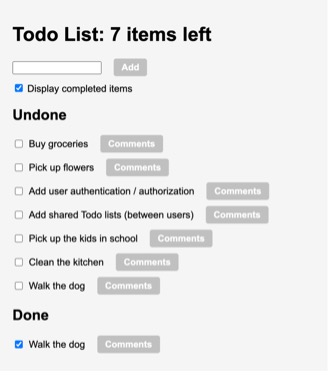
\includegraphics[width=\textwidth]{Pictures/Picture1.jpg}
    \end{subfigure}%
    \begin{subfigure}{0.38\textwidth}
        \centering
        
\includegraphics[width=\textwidth]{Pictures/Picture2.jpg}
    \end{subfigure}
    \caption{UI of the Todo-application}
    \label{fig:todo}
\end{figure}

\noindent The approach was originally tried out with ChatGPT in a POC where an application was developed from scratch up to production. The application manages todos~\cite{Freeman2013}, with the UI in Figure~\ref{fig:todo}.\footnote{See http://formalit.dk/portfolio.html for github links and presentation.}  The POC had these parts and steps:
\begin{itemize}
    \item UI built with React
    \item API built in Javascript running on Node.js
    \item Data layer with Postgres database
    \item UI hosted as Azure static web app
    \item API hosted as Azure app service
    \item Code in GitHub
    \item Automatic deployment on merge of each PR
\end{itemize}

\noindent In later projects in our daily work we have used {\em Cursor} as the agentic IDE~\cite{Cursor_2023}. Some variants would be {\em Github CoPilot}~\cite{GitHubCopilot_2023} or {\em Devin}~\cite{Devin_2023}. In Cursor one can choose between various LLMs, we prefer GPT-4o~\cite{GPT40_2023}, some other options are some Claude~\cite{Claude_2023} and Gemini~\cite{Gemini_2023} models.

The remainder of the paper is organized as follows. We first explain the overall approach. The follow sections with the detailed steps of the approach, drawing examples of the use of LLM from the POC and the use of agentic IDE from in later experiences.  There is also a section with the details of the POC and one with details of later examples.

\section{Overall Approach}
The approach can be briefly explained as follows. Imagine you are senior lead developer for a team of, say, five developers, excluding yourself. The developers are junior, medio or senior and front-end, back-end or full-stack developers.

Imagine you actively manage the team by providing functional requirements to each individual developer where work is organized in sprints. For the UI development it is in the form of screen shots (e.g., Figma) and user stories. For the DB layer, it will be by specifying tables and columns with primary and foreign keys. This carries over to the CRUD part of the API layer, which may also include, among others, validations, business logic, calculations and authentication and authorization.

Also imagine that the application has a skeleton which expresses how to deal consistently with common themes. For the UI, it will be how to manage state, where to place call-back handlers, how to call APIs, etc. For the API it will be, e.g., your selected separation into controller, service, and repo layers and how to manage ORM directly or by 3rd party libraries. The skeleton may come from you or the developers (or as the first step of the approach).

From this point on you delegate features to the developers. You review each pull request (PR) from each developer, possibly asking for revision of the code, e.g., to ensure consistency and completeness. After approving PRs, the API test and UI tests are automatically run and any errors are identified and communicated to the developers, who will fix them and start another cycle of the loop. The tests are extended by the developers to cover their new functionality.

Now imagine ChatGPT acting as each developer. The prompts correspond to the delegation to developers, and the generated answers make up the PRs. Finally realize that Cursor handles the communication with ChatGPT and implements the actual PRs by updating your files and issuing terminal commands for running the build, committing and pushing to github, etc.

The different steps of the approach are explained in the following sections.

\section{Set Up The Project}
This step is usually required only once for a range of sprints leading to one or more applications in the same company, so it does not have to be super-efficient. Nevertheless, ChatGPT can create a step by step instruction on how to set up the project and Cursor can actually do the steps.

\mybox{\textbf{Lesson 1:} ChatGPT can provide tutorials tailored to your application on how to accomplish any tasks. Cursor can actually do the steps on your laptop.}

\noindent The local development environment must be efficient to work with because it is crucial to have a fast loop of getting pull requests from ChatGPT, and letting cursor run the  UI and API tests and identify and fix issues.

\noindent In the POC, we used a mixture of ChatGPT and \cite{Freeman2013} to provide basic setup of IDE and project files. There were a couple of issues with versions and dependencies, but they were not difficult to fix. We set up the code in a GitHub repository, which made it easy to backtrack when ChatGPT produced undesirable code. In other examples, we have used Cursor to set up Python projects handling existing and new dependencies very efficiently.

\mybox{\textbf{Lesson 2:} Set up the local development environment to efficiently support the iterations with ChatGPT and Cursor. It will be a one-time cost. Always begin with a GitHub repo to avoid loosing code by deletion or overwrites.}

\section{Get Started With Development}
Fowler\cite{Fowler2023} celebrates an approach, where you first communicate to ChatGPT an overall plan of steps that should be carried out before going into details.

The way we see it, this plan may reside in the mind of the team lead, who delegates parts to the individual developers without each of them necessarily knowing the entire plan.

For instance, for the POC, we could start with the code to generate the relevant database tables, then create the needed API, and finally create the UI.

In fact, we recommend following the three steps in this order (DB, API, UI) for one feature, and then repeat them for each new feature. There are many reasons why this iterative development is a good idea in conventional projects without ChatGPT, and they carry over to the new way of developing software with ChatGPT. For instance, it avoids the useless code Gewirtz\cite{Gewirtz2023a} experienced.

\mybox{\textbf{Lesson 3:} Split the development into sprints and user stories, like you would with a team of developers. Then proceed sprint by sprint, user story by user story, for the same reasons as you normally do.}

\mybox{\textbf{Lesson 4:} In Sprint 1, establish the fundamental architecture of the application, for instance a UI layer, an API layer, and the DB layer developed well enough to cover a small feature. The architecture should not only align to functional and non-functional requirements, but also to the team size and  experience.}

\section{Create The Data Model}
In a conventional project we would recommend developing a feature by doing the UI and API simultaneously, because each aspect helps to validate the other and together, they deliver a complete feature. The DB part can probably be done by the API developer, both are part of a typical back-end profile's capabilities.

With ChatGPT and a single development lead, the separate parts UI, API, DB are sequential, and we recommend doing them in the order DB, API, UI, since the UI needs the API, which needs the DB.

So, first you generate the data model. Either you already know the entire data model, or you know only part of it. In any case, as already mentioned, you should start with one or two example entities and create the DDL or migrations, depending on your preferred approach, to confirm that you get the expected results.

Some people recommend postponing the DB layer, for various reasons. For instance, it is argued that the DB layer can change from relational to NoSql. Also, it is emphasized that it is important to solicit quick feedback from product management, which suggests emphasizing the UI.

However, in our experience most applications have a data model, relational or otherwise, and understanding this model is the key to have a solid basis for the entire application.

\textbf{Lesson 5:} Except for mock-ups, UI experimentation and hobby projects, most sprints should start by implementing the data model of the feature.

\section{Create The Api}
Having created the necessary tables for a feature, you can proceed with the API.

As mentioned, you should first generate a small part, verify what ChatGPT provides and make sure that it meets expectations. Although it is impressive how accurate and
correct ChatGPT's answers often are, also in our experience, they are not flawless. Mistakes encountered include basic oversights (for which it always politely apologizes), but occasionally also more fundamental flaws that indicate that it completely misses the point.

\textbf{Lesson 6:} ChatGPT's answers should be evaluated like they come from another (sometimes less experienced) person, rather than from a flawless machine. The human developer who integrates ChatGPT's responses into the application remains liable.

If you are not content with the results that ChatGPT provides, it is often advisable to iterate to get what you want. If you are confident that the code is correctly structured, you could go for the overall thing in a second round after the initial sprint and relevant follow-up shows that the code is functionality correct and well-structured.

Also, if you are delivering to a company that already has policies for how the code should be structured you can ask ChatGPT that the code structured in that way.

For instance, do you have multiple layers with controller, service, and repo, or less than that. In general, keep things as simple as possible. The fewer moving parts and the fewer proprietary add-ons that ChatGPT has no knowledge about, the easier it will be for ChatGPT to get it right. Besides, you can always get ChatGPT to rewrite the 
files later if you decide.

Remember the API is not just happy scenario, so provide instructions about error handling, return codes, etc. For instance, in the POC, the API server could initially crash when there was some issue. So we asked ChatGPT to wrap each call in a try catch, and return 200 or 500 depending on whether an error was encountered or not. We should note that on several other interactions, ChatGPT actually suggested that error handling should be part of the implementation and provided examples of how to do it.

\textbf{Lesson 7:} When starting the API, get a simple server running with a simple example and make sure you are happy with it to some level of maturity. There may be some production hardening missing that can be covered latter, but the basic structure should be correct and satisfactory.

\section{Create The Ui}
Having established DB and API for the first sprint, proceed to the UI. This is where we see the largest difference working with ChatGPT, compared to the conventional approach.

With a developer you will typically show a screen shot of some sort, maybe Figma wireframes produced by product management, accompanied by some explanations.

Since ChatGPT does not support visual input yet, we need to rely on only explanations. This makes it more difficult to explain details like horizontal and vertical layout, and adds to the possibilities for incorrect interpretation, leading to incorrect or suboptimal results.

We therefore prefer to tap into the developer's fine- grained process of progress. When confronted with a feature with a page with multiple controls and fragments, he should begin with some simple subset and get it to work to create a basis. After this, he can add the remaining elements one by one or in small groups in an iterative way.
Similarly, when we instruct ChatGPT, we first ask for a simple version of the page, confirm it works, and then add further elements.

This process helps keep to the code and the development process – here meaning the interaction with ChatGPT – under control. You get small parts, which can easily be validated and tested. In other words, we do not end up with legacy code, contrary to the claim of Loukides\cite{Loukides2023}.

\textbf{Lesson 8:} When working with ChatGPT on User Interface, ask first for a simple version. Then add remaining controls one by one or in small groups.

We will later discuss how we can scale the development of UI to a more efficient process where the UI is explained in a semi-formal way.

\section{Intermezzo: the POC In Detail}
In [1] the development of a Todo application proceeds from UI to API (contrary to our recommendation, but the book is about React, so it makes sense). Let's follow that path and see how ChatGPT works it out.

We start with the standard React application obtained by running npx create-react-app todo, which was part of the project setup. After this, we ask ChatGPT to create the contents for the files we already have as dummy versions:

When you ask ChatGPT to generate code he will often give you examples and leave to you to complete the details. However, it is much faster if ChatGPT simply does it all. So, we ask for full contents of the files.

\textbf{Lesson 9:} Ask for full contents of files. It speeds up the process.

For the above request we get this response:

ChatGPT goes on with the contents of each file.
   
Sometimes there can be slight imprecisions in ChatGPT's responses. For instance, about the name of entities, file locations, etc. That's why it's good to have a working dummy application where files are correctly named and stored in locations that are consistent.

\textbf{Lesson 10:} When starting the interaction with ChatGPT, have a dummy application working.
Next, we want to indicate whether todos are done.

ChatGPT responds with the changes.
    
We confirm the code is working and move on to the next missing part.

ChatGPT responds:

and breaks it into parts as usual.
  
We are ready for the last part. The application (focused on UI) now has most of what is shown in Section 1, except the Comments page, the
styling, and a few details. Now we move on with the API.
    
After we try out the end points and confirm they are working we can make the UI use them.

Let's see how to have simple manual test.
  
As mentioned, sometimes ChatGPT will generate code that does not work. In many cases it is because of small details like not naming paths in json correctly (because of lack of context). In general, ChatGPT is pretty good at helping with the issues.

In this case we have this error. ChatGPT responds:

The advice turns out to work. In general, such advice should be confirmed by checking with other sources. Although, code is contributed by ChatGPT, you should see yourself as liable for it. See [7] for more on this aspect and [6] for questions about copyright regarding the code. Also notice that confidential code or information should not be shared with ChatGPT as observed in [3].
  
\textbf{Lesson 11:} ChatGPT may generate code with issues for various reasons, e.g., because we did not ask explicitly to avoid them or because he made an interpretation that is incorrect in our context. In such cases, simply ask for help; most of the time he will be able to (help) resolve the problem.

At this point, repeated testing reveals some new errors, ChatGPT replies with new versions where the errors are solved, and the ping-pong game continues for a little while until the code eventually works. Again, the trick is to get ChatGPT to do the work and keep providing the updated component in full, rather than to provide instructions for the developer to address these himself.

\textbf{Lesson 12:} As mentioned, ChatGPT may generate code with errors but getting it to fix them is quicker than writing the code yourself, which may also introduce errors that may take time to find and resolve.

Interestingly, at the end, the todo items are back in single list, rather than two different for done and undone. ChatGPT lost some context along the way in the new issues, as others have reported, and we had to get him back on track. Also, we had to instruct him that the API should be called to mark todo items done or not done.

\textbf{Lesson 13:} ChatGPT may generate code with problems that were solved earlier in the dialog. You need to test what he returns at every step and ask errors to be fixed.

We will say more about automatic testing later. It's finally time to get the DB layer done.

He politely responds.

And he continues:

Then follows some more ping-pong about
• The user the API should connect to the DB with.
• Handling "done" information in post endpoint.

\textbf{Lesson 14:} Be as precise as you can in stating what you need from ChatGPT. Whenever you omit details, ChatGPT may do something else than you expect.

Not long after this we have an application that works with all three layers. However, there are still many details

missing before the application is appropriate for production. For instance, the server code is in one big file which does not scale for a bigger API. Also, there is no error handling. We return to these and other issues later.

TODO
\textbf{Lesson 15:} If ChatGPT is lacking context, he may make assumptions instead of asking for clarifications. You can circumvent this by explicitly directing him initially to ask clarifications.

Areas where ChatGPT's help proved useful or invaluable:
• Rewriting the security and authentication layer,
by replacing a proprietary component with an
approach based on JWT tokens.
• Migrating from simple sequence-based primary
keys to primary keys that follow the Twitter
Snowflake pattern.
• Implementing new frontend views based on the
existing application structure.
• Hunting down and resolving issues.
• Providing feedback and structuring the pros and
cons for engineering tradeoffs.

One example where ChatGPT significantly sped up issue resolution is the following. After modifying the primary keys in the database from natural numbers (1, 2, 3...) to Twitter Snowflake style (e.g., 1139459444921196544), in certain situations the frontend could not find the data required, even though it was in the database.

When we presented this issue to ChatGPT, within seconds he explained that in the frontend our ids (modelled as long in our backend) should be represented as string to avoid rounding for the large numbers that our indexes are. It is our estimation that isolation of such an issue without ChatGPT could easily have taken a full day for an experienced developer.

Also, confronted with situations that required an engineering trade off, ChatGPT provided valuable
1 Material UI, via https://mui.com.
overviews of the pros and cons. It should be noted that on several instances – following the DRY principle – we deviated from the suggestions, e.g., by implementing a common feature in an AbstractService class, rather than in each service itself.

\section{Create the Styling}
If the DB layer is seen as the nitty-gritty details below the API, the styling are the nitty-gritty details above the UI.

Explaining styling to ChatGPT is even worse than explaining the basic layout of pages.

There are various offerings that can generate artifacts from drawings or even Figmas. They may gain traction onwards. We tried out one with not the results we needed. For instance, it was not possible to generate React code. We do not rule out that such tools exist, but the feature had been removed from the tool we tried out.
Instead, we tried to get ChatGPT to generate CSS for Example 3. He correctly used an HTML grid and got the basic layout right, but adjusting the details turned out to be 
impossible after 2-3 iterations.

At this point we reverted to classical techniques and studied HTML and CSS documentation and manually did the needed adjustments.

\textbf{Lesson 16:} Sometimes, several iterations do not bring you closer to a solution. In these cases, consider reverting to classical techniques, like Googling, Stack Overflow, YouTube demos, reading the documentation, etc.

As the discipline of coding with ChatGPT evolves, it can be expected that efficient approaches will be developed to deal with UI specification, CSS, SASS, etc.

By the way, the approach to styling is in general evolving. Initially you did the styling in HTML, then came CSS, and these days you have SASS or even technologies such as Tailwind CSS. You should instruct ChatGPT to deal with styling at the level fit for your application needs.

Also, you can request that controls be used from standard libraries such as material-ui1 or more recent approaches like Tailwind CSS, etc. However, notice that so far, ChatGPT is not trained on material to the current date, so he may prefer approaches that are not fully up to date.

For instance, In Example 2, when we later created a basic application based on Next.js, he was expecting a file
 
structured based on the classical router with the pages directory. In contrast, the default option when creating Next.js applications these days uses the new App router.
\textbf{Lesson 17:} ChatGPT currently does not know about knowledge published after September 2021.

\section{Create the Tests}
As mentioned, ChatGPT – like most developers – generates code with errors, even errors that were previously fixed.

The most efficient approach to dealing with these is to have two slim test suites, one that tests the API and one that tests the UI.

For the POC, the UI test was produced with Puppeteer. It has these steps:
\begin{itemize}
    \item Open browser and go to main page.
    \item Click Show completed todos.
    \item Type into the item input field.
    \item Click the "Add" button.
    \item Confirm the new item is there.
    \item Click the new item's check mark.
    \item Check the new item is now in the done list.
\end{itemize}

The test ends by deleting the new item using the API.

When adding new functionality from ChatGPT we check locally that the UI test runs before merging the pull request. We also manually check the new feature works and add a UI test for it. For the new feature, we prefer to first check it manually, so that if the automatic test fails, we know the problem is with the test.

The API test was a sequence of API calls in code using axios (a HTTP client library) imitating a UI interaction. Again, the test ends by deleting the data it has added using the API.

\textbf{Lesson 18:} ChatGPT generates several errors. It is valuable to have a slim UI test and API test that can be run locally before merging pull requests.
We do not bother to mock database or service layer. Since we have the development environment running locally, we can rely on it as long as the tests:
\begin{itemize}
    \item Do not make any assumptions about the condition of the database on entry.
    \item Leave the database in the same condition on exit as it was in on entry.
\end{itemize}

\textbf{Lesson 19:} By keeping the tests slim, lightweight, and direct, they do not need to be time consuming and can be a good way of testing pull requests from ChatGPT.
The tests were written manually, because we wanted to make sure the code from ChatGPT did what we asked. Some people prefer to let ChatGPT generate the tests, but we see a risk that when ChatGPT gets something wrong in code, he will get the same thing wrong in tests. Indeed, errors were frequently about aspects that were not sufficiently well communicated, e.g., field names.

Nevertheless, we are open to the approach that you start by having ChatGPT create the tests and review that they capture what you want.

\section{Refactor Out Common Parts}
When you ask ChatGPT to generate some code, he will try to satisfy your requirements, but in many cases, he will refrain from satisfying your untold requirements, even if you regard them as common sense.

To be fair, when he generates some code, he will sometimes tell you that this is just an example, and you also need to take into account some list of considerations. But at the end of the day, you cannot assume he satisfies non-functional requirements that you do not mention.

An obvious example is when the same code occurs in multiple places. In this case we want to factor it out.

For instance, in the POC we added the possibility to have some fields of the todo encrypted in the database (GDPR, you know the drill), so that developers cannot see the contents of the fields when they access the database.

The code to encrypt when storing and decrypt when fetching should not be replicated to the handler of each end point. There should rather be utility functions that are called from the API endpoints handlers:
 
You can handle these requirements up front when asking code to be generated or refactor along the way by explaining to Chat GPT the current files and their contents and the required refactoring.

\textbf{Lesson 20:} As you review the PRs from ChatGPT, keep an eye on parts of the code that could or should be refactored. Either do the refactoring yourself or ask ChatGPT to do it.

In general, we want to limit refactoring to a reasonable limit and only allow it when it has a tangible result and good balance between effort and benefit not based solely on speculation.

But some refactoring just has to be done. Like having significant chunks of code that is replicated verbatim in many methods pulled out to a method.

\section{Design The File Structure}
When you design your application with ChatGPT there are typically two different approaches:
\begin{itemize}
    \item You did this many times and have a clear idea about the major design and architecture choices.
    \item You are doing this in an exploratory manner.
\end{itemize}

Both approaches have their merits. If you work in the explanatory way, you should expect to do refactoring along the way. ChatGPT can provide advice on the structure and even generate the files. For instance, at the end of the POC, the UI looked like this:

Similarly, the API looked like this:

Have a clear structure for the files of your application in mind from the beginning and communicate it to ChatGPT in your prompts, or be prepared that you or ChatGPT should refactor the code along the way to replace a single file by a set of files each of which covers a feature.

Similarly, be prepared that as more complexity arrives, a single layer may be split into several layers, e.g., for the API as service, controller, repo, etc.

\textbf{Lesson 21:} You are responsible for ensuring that the file structure of the application is manageable. Define it from the outset or refactor it (with the help of ChatGPT) along the way.

\section{Keep The Code Under Control}
As mentioned, you should be prepared to refactor. What was said in the preceding section was about splitting large files into smaller more manageable files, e.g., 
splitting a single file with the handlers for all end points into separate files grouped by entity or entity groups.

Also, we have mentioned that every response from ChatGPT should be seen as a pull request. That way no code ever enters the code repository without some sanity check. You don't need to read every single line, but you need to gain confidence that the code follows the philosophy and guidelines that you are trying to enforce. What we can add to this is that the code should be structurally consistent. This means that how different kinds of functionality or logic is structured or organized should be the same from feature to feature.
  
 For instance, in the POC, the page fragments were initially classes. However, when we added the page for adding comments on todos, we introduced version 6.14.1 of react-router-dom and had to make use of the useParams and useNavigate hooks for retrieving the URL parameters and for navigation, respectively. And this led to some classes being reformulated as functions. In this case, it is preferable that all the components are functions.

The reason ChatGPT got us into the classes formulation in the first place may be that this was the most widespread method during the period of documents that ChatGPT has 
been trained with.

\textbf{Lesson 22:} Keep the code consistent. ChatGPT may change structure of the code he generates when new requirements from you become clear. You should refactor the previously generated code (make ChatGPT do it) when this happens. Consider code measurement tooling at the end of the project to confirm and document consistency.

It is claimed in [2] regarding the code generated by ChatGPT that "For all practical purposes, it's 'legacy code,' even if it's only a few minutes old." As hinted at earlier, this does not apply to the approach described here:
1. Developers may leave you and are not there to explain their code. ChatGPT and related technologies are here to stay and will improve over time.
2. You must review the code from ChatGPT and adopt it as your own code. So long as you are there, it's not legacy.

\textbf{Lesson 23:} See the code by ChatGPT as your code. You must be able to account for it. That way it has same value as code developed by you or your developers.

\section{Go To Production}
So, you have your code generated by ChatGPT and it does what you asked. The UI tests run, the API tests run, all good. But are you ready for production?
If you are an experienced developer, you know many things are missing. For instance, you may need a penetration test to ensure that you did everything to correctly handle 
security-related HTTP-headers, SQL injection attacks, cross-site scripting etc.

Actually, you can ask ChatGPT what is required from, say, an API before it is mature for production, and he will help you:
This provides a checklist, which can be elaborated upon as needed. If you have any questions, you can ask again. For instance, how do you check if the API is vulnerable to SQL injection, ask and he will help you test it.

For example:
  
Again, such responses should be checked with alternative sources.

\textbf{Lesson 24:} The code that you get from ChatGPT may not be ready for production, but he can help you understand what needs to be checked and how, and which changes are needed as a result of the checks.

\section{Set Up The Prod Environment}

Like with the development environment, we eventually need a production environment.

For the POC, we used Azure Postgres for the database layer. For the UI and the API, we initially used Azure App service. For the UI, upload took ages and there were some issues getting it to work. After a while we backtracked and looked for demos of how to deploy a React application on Azure and changed to Azure static web app, which ran much smoother.

We need some additional DevOps work. For instance, as mentioned, for the POC we set up a GitHub repository and had automatic deploy to the environment when there are commits to the branch.

Depending on your organizational setup, number of applications to develop, etc. you may find it desirable to script provisioning of your environments as often done.

\section{Scale With Formalism}

Once you start doing multiple applications with ChatGPT, it becomes natural to optimize the communication.

One interesting possibility is that you can train ChatGPT with training material yourself. That is, you can give examples of what prompts you provide and at the same time provide the desired answer.

This can be used to train him to deal with formal specifications of UI. For instance, you provide a text representation of a UI by listing all the components of a page including alignment margins etc. and show the HTML or React code you expect.

We have already pursued this approach some way but leave as future work to report on it in detail.

\textbf{Lesson 25:} Formalize your communication with ChatGPT with initial training. That way the communication can hopefully be way more efficient and less ambiguous.
Indeed, it's been a goal in the software engineering community for decades to formalize development. We create a specification in some formal language, and the system generates the code which is provably correct with respect to the specification.

So far this did not become a widespread practice in the community. We can speculate that the following reasons apply:

1. It is very difficult to translate the nature of the problem that a solution will solve to a formal specification in one go. If this was easy, waterfall development would have been more successful.

2. Your formal specifications cannot embrace the needed functionality of your target applications unless they are as complicated as the target language and then what have you won?

3. Due to the complexity of the specification language, you will make errors in your specification that are as severe as errors in the generated application.
What became possible overnight is to provide the specification that you can invent yourself and train ChatGPT in. And the remaining requirements that do not fit conveniently into the specification can be mentioned informally, they will be taken into account by ChatGPT. We look forward to exploring this possibility further.
  
\section{Scale With Developers}
Remember the five developers that left us? Now they are back.

Today the development lead, as we envisage the role, coaches the developers, and supports them in how they code. Replacing them with ChatGPT you may think they are gone.
But when this shift is made, the development lead becomes the bottleneck. The obvious way out is that the development lead does not coach ChatGPT in how to code. He 
coaches the developers in how they coach, work, and interact with ChatGPT.

Software development has fundamentally changed since the introduction of ChatGPT. Both the industry as a whole and every practitioner in it is trying to understand the implications in this interesting era.

Our approach assumes that there are experienced developers; it is an interesting question how humans can continue to build and retain knowledge and skills if ChatGPT is to take over the bulk of coding. Will this not also lead to an erosion of understanding? Also, we assume ChatGPT has been trained on material regarding coding in given language. Again, for a new language, how can this happen for a new language if ChatGPT itself is supposed to do the coding? Many questions remain.

\section{Limitations}
ChatGPT can help you, but there are also limitations:
\begin{itemize}
    \item ChatGPT may be periodically unavailable.
    \item He accepts a limited number of prompts in a fixed amount of time.
    \item There have been reports of degradation of his responses, at least for ChatGPT 3.5
    \item ChatGPT is an echo chamber: he will provide what knowledge is agreed by most people. If you have unique shortcuts based on experience, he may not agree.
    \item ChatGPT does not know about recent develops, such as new languages and frameworks, etc.
\end{itemize}
In practice we have so far not found these limitations to severely restrict the benefits of using ChatGPT.

\section{Conclusion}
We have outlined an approach to developing mature, production-ready, maintainable full stack applications from scratch with ChatGPT. Based on our examples we estimate the productivity improvement to be a factor between 2 and 5.

The method does not work out of the box, you must adopt various practices. Most importantly, you should work with ChatGPT the same way as you do today with developers:
\begin{itemize}
    \item Create the architecture and features in sprints.
    \item Regard the contributions by ChatGPT as pull requests that you should review.
    \item Implement lightweight regression testing for UI and API to confirm that refactoring and adding functionality by ChatGPT does not break anything.
    \item Get ChatGPT to refactor along the way to turn duplicated code into methods and to implement other patterns that you observe the need for in the pull request reviews.
\end{itemize}
Our hands-on experiments suggest that ChatGPT, guided the right way, can contribute working code, identify relevant libraries and frameworks, identify the source of bugs, suggest methods to mature and secure the application, and contribute in many other ways that save time and money, and improve quality and time-to-market.
ChatGPT can make mistakes, but so can developers, professors, and textbooks. When you receive advise that you cannot confirm satisfactorily yourself, it is always good to double check with an alternative authoritative source. For instance, when putting a new application to production, it is a good idea to get an external company to conduct a penetration test, whether the application development got help from ChatGPT or not.
At the end of the day, we think of ChatGPT as a developer that read all the relevant documents and pieces of code that exist for that language in question and gives the best answer to your question at hand. In our experience, ChatGPT and related technologies should be evaluated and used today, since their potential to reduce time-to-market and increase efficiency, while increasing quality, is vast.
In most cases, ChatGPT can do things faster than you can. Whenever getting caught up in anything that seems remotely routine, ask yourself this question: Shouldn't I get ChatGPT to do this?

A revolution in software development has started. Are organizations ready to adopt and reap the benefits...?

\appendix
\section*{Appendix}
\begin{figure}[h]
    \centering
    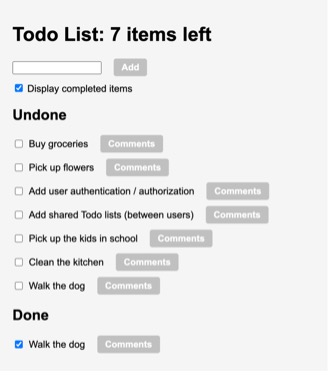
\includegraphics[width=0.5\textwidth]{Pictures/Picture1.jpg}
    
\includegraphics[width=0.5\textwidth]{Pictures/Picture2.jpg}
    \caption{Description of Picture1}
    \label{fig:picture1}
\end{figure}
\begin{figure}[h]
    \centering
    \caption{Description of Picture2}
    \label{fig:picture2}
\end{figure}
\begin{figure}[h]
    \centering
    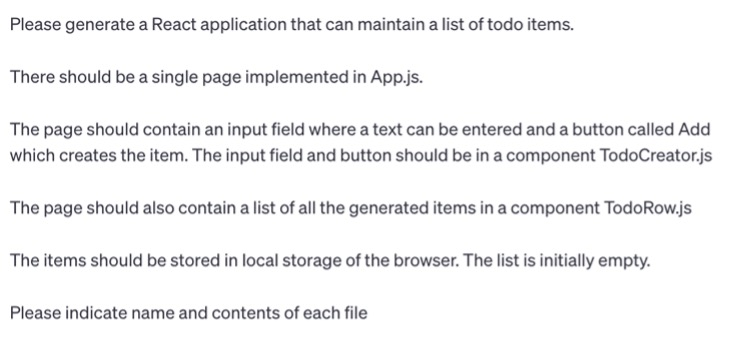
\includegraphics[width=0.5\textwidth]{Pictures/Picture3.jpg}
    \caption{Description of Picture3}
    \label{fig:picture3}
\end{figure}
\begin{figure}[h]
    \centering
    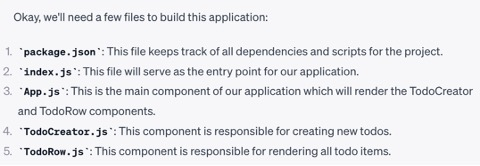
\includegraphics[width=0.5\textwidth]{Pictures/Picture4.jpg}
    \caption{Description of Picture4}
    \label{fig:picture4}
\end{figure}
\begin{figure}[h]
    \centering
    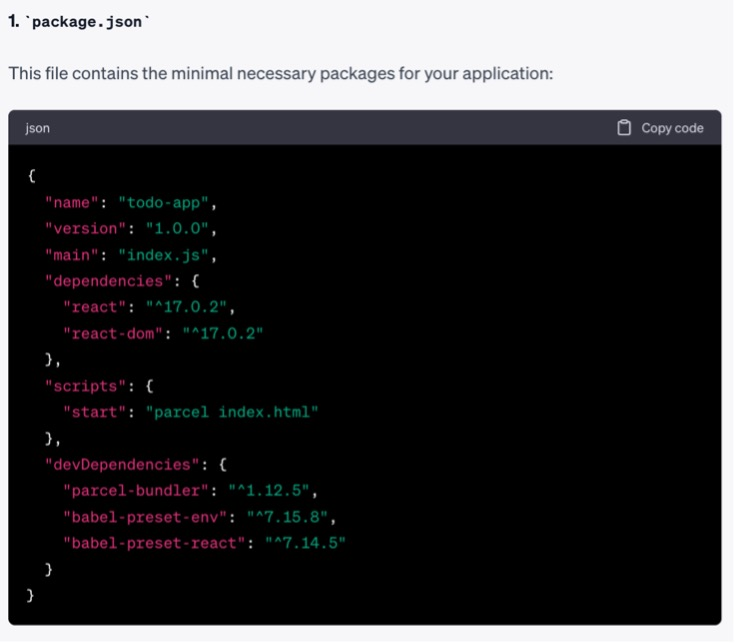
\includegraphics[width=0.5\textwidth]{Pictures/Picture5.jpg}
    \caption{Description of Picture5}
    \label{fig:picture5}
\end{figure}
\begin{figure}[h]
    \centering
    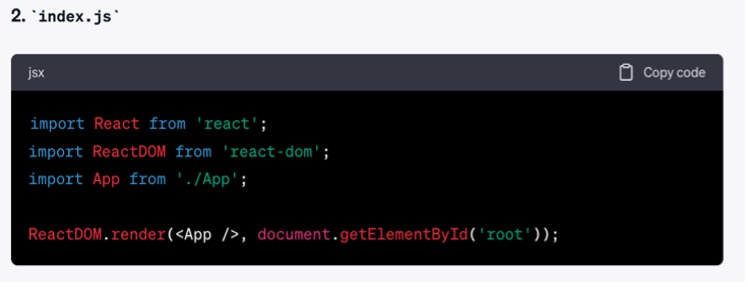
\includegraphics[width=0.5\textwidth]{Pictures/Picture6.jpg}
    \caption{Description of Picture6}
    \label{fig:picture6}
\end{figure}
\begin{figure}[h]
    \centering
    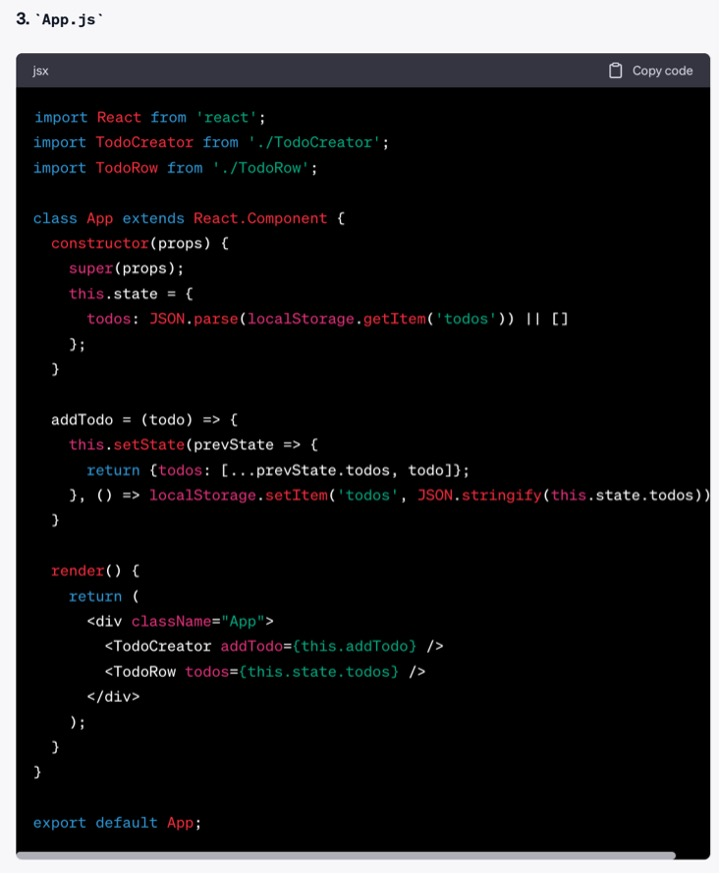
\includegraphics[width=0.5\textwidth]{Pictures/Picture7.jpg}
    \caption{Description of Picture7}
    \label{fig:picture7}
\end{figure}
\begin{figure}[h]
    \centering
    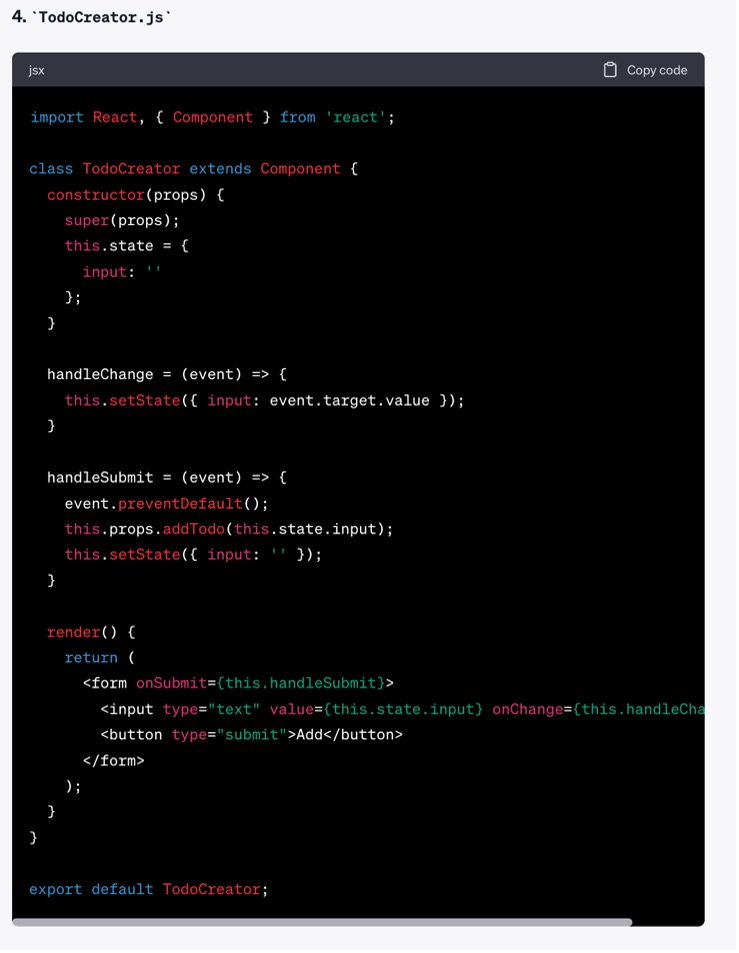
\includegraphics[width=0.5\textwidth]{Pictures/Picture8.jpg}
    \caption{Description of Picture8}
    \label{fig:picture8}
\end{figure}
\begin{figure}[h]
    \centering
    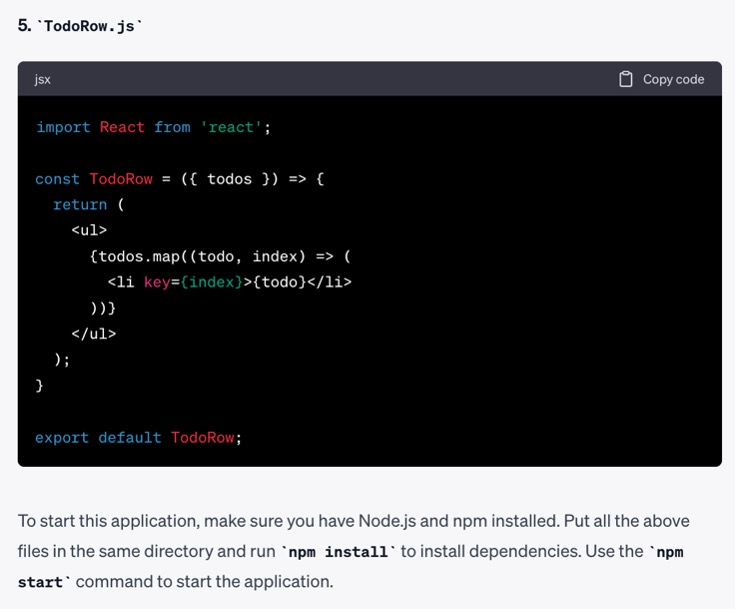
\includegraphics[width=0.5\textwidth]{Pictures/Picture9.jpg}
    \caption{Description of Picture9}
    \label{fig:picture9}
\end{figure}
\begin{figure}[h]
    \centering
    
\includegraphics[width=0.5\textwidth]{Pictures/Picture10.jpg}
    \caption{Description of Picture10}
    \label{fig:picture10}
\end{figure}
\begin{figure}[h]
    \centering
    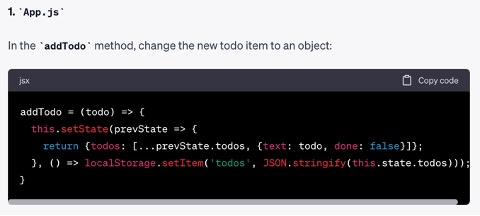
\includegraphics[width=0.5\textwidth]{Pictures/Picture11.jpg}
    \caption{Description of Picture11}
    \label{fig:picture11}
\end{figure}
\begin{figure}[h]
    \centering
    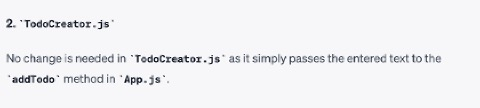
\includegraphics[width=0.5\textwidth]{Pictures/Picture12.jpg}
    \caption{Description of Picture12}
    \label{fig:picture12}
\end{figure}
\begin{figure}[h]
    \centering
    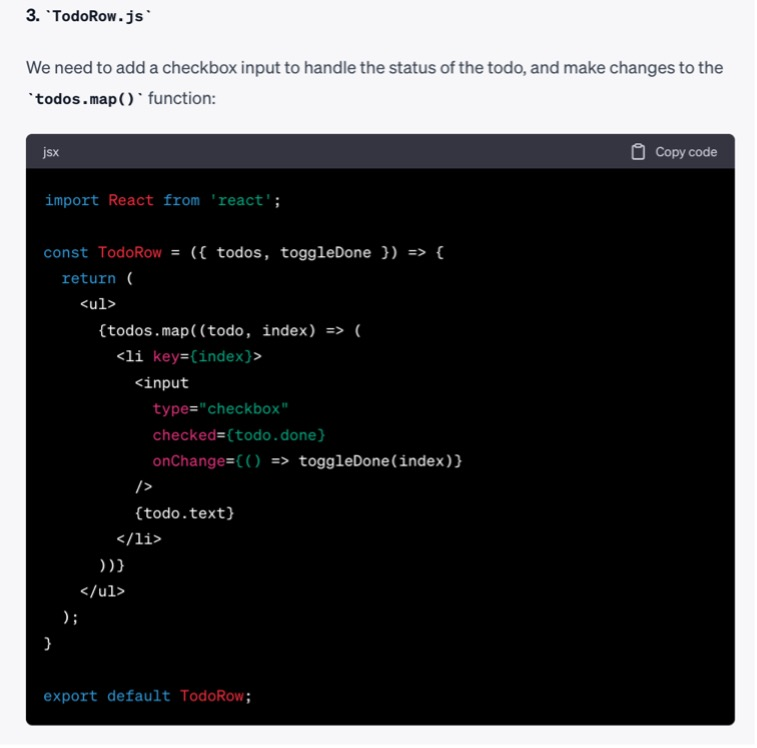
\includegraphics[width=0.5\textwidth]{Pictures/Picture13.jpg}
    \caption{Description of Picture13}
    \label{fig:picture13}
\end{figure}
\begin{figure}[h]
    \centering
    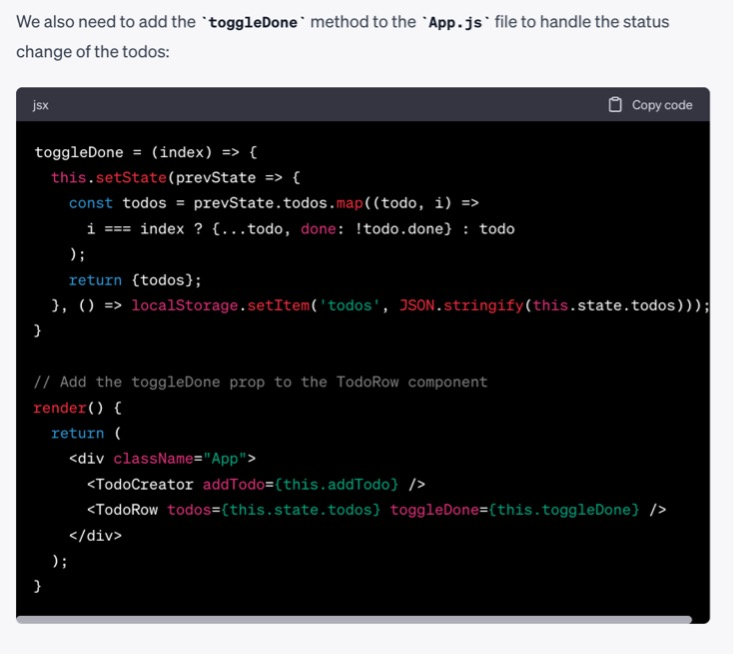
\includegraphics[width=0.5\textwidth]{Pictures/Picture14.jpg}
    \caption{Description of Picture14}
    \label{fig:picture14}
\end{figure}
\begin{figure}[h]
    \centering
    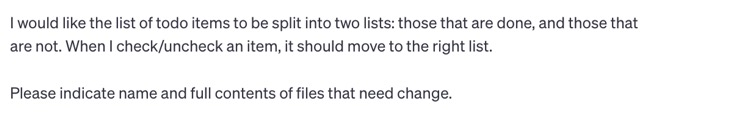
\includegraphics[width=0.5\textwidth]{Pictures/Picture15.jpg}
    \caption{Description of Picture15}
    \label{fig:picture15}
\end{figure}
\begin{figure}[h]
    \centering
    
\includegraphics[width=0.5\textwidth]{Pictures/Picture16.jpg}
    \caption{Description of Picture16}
    \label{fig:picture16}
\end{figure}
\begin{figure}[h]
    \centering
    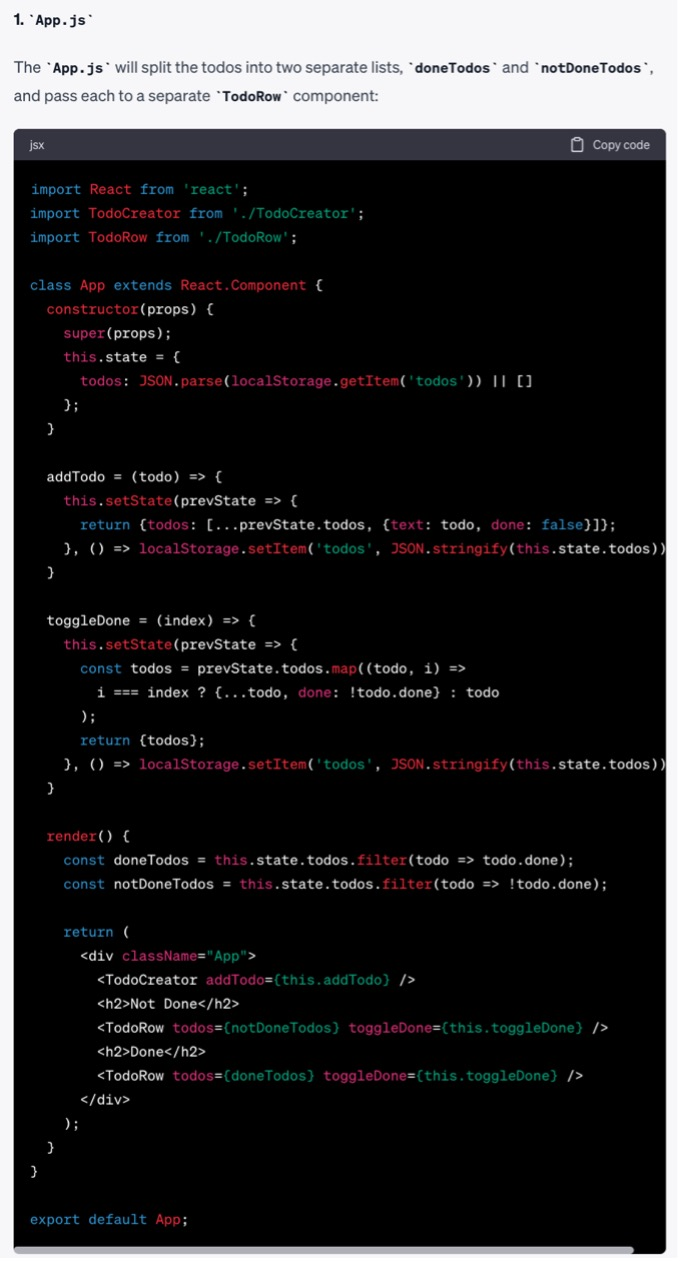
\includegraphics[width=0.5\textwidth]{Pictures/Picture17.jpg}
    \caption{Description of Picture17}
    \label{fig:picture17}
\end{figure}
\begin{figure}[h]
    \centering
    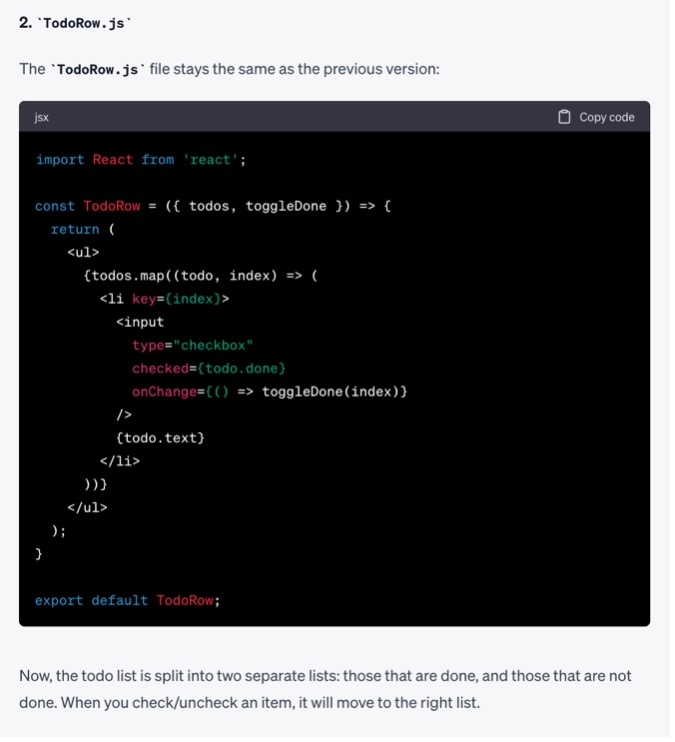
\includegraphics[width=0.5\textwidth]{Pictures/Picture18.jpg}
    \caption{Description of Picture18}
    \label{fig:picture18}
\end{figure}
\begin{figure}[h]
    \centering
    
\includegraphics[width=0.5\textwidth]{Pictures/Picture19.jpg}
    \caption{Description of Picture19}
    \label{fig:picture19}
\end{figure}
\begin{figure}[h]
    \centering
    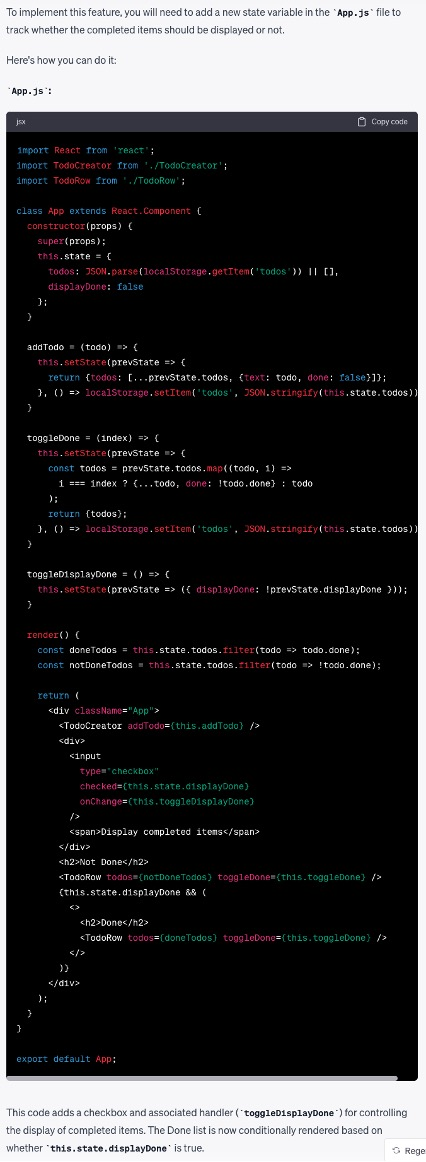
\includegraphics[width=0.5\textwidth]{Pictures/Picture20.jpg}
    \caption{Description of Picture20}
    \label{fig:picture20}
\end{figure}
\begin{figure}[h]
    \centering
    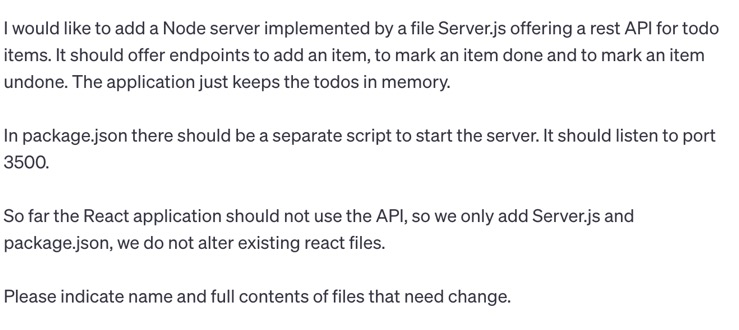
\includegraphics[width=0.5\textwidth]{Pictures/Picture21.jpg}
    \caption{Description of Picture21}
    \label{fig:picture21}
\end{figure}
\begin{figure}[h]
    \centering
    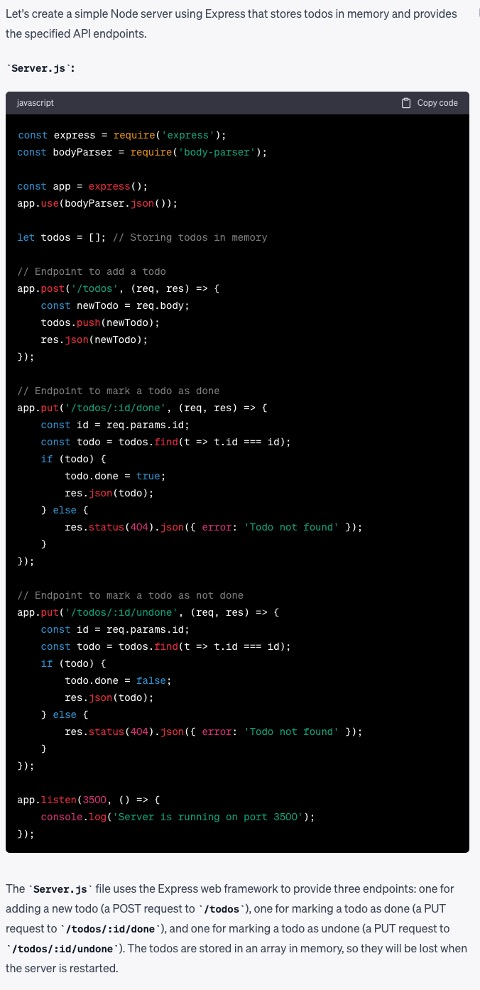
\includegraphics[width=0.5\textwidth]{Pictures/Picture22.jpg}
    \caption{Description of Picture22}
    \label{fig:picture22}
\end{figure}
\begin{figure}[h]
    \centering
    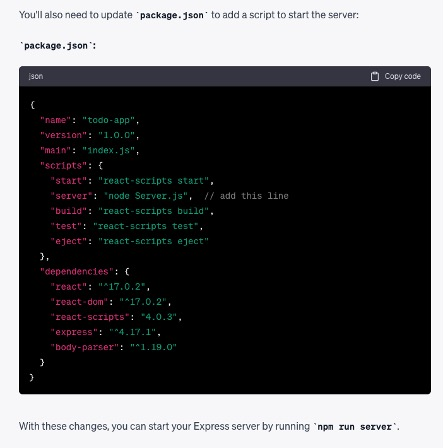
\includegraphics[width=0.5\textwidth]{Pictures/Picture23.jpg}
    \caption{Description of Picture23}
    \label{fig:picture23}
\end{figure}
\begin{figure}[h]
    \centering
    
\includegraphics[width=0.5\textwidth]{Pictures/Picture24.jpg}
    \caption{Description of Picture24}
    \label{fig:picture24}
\end{figure}
\begin{figure}[h]
    \centering
    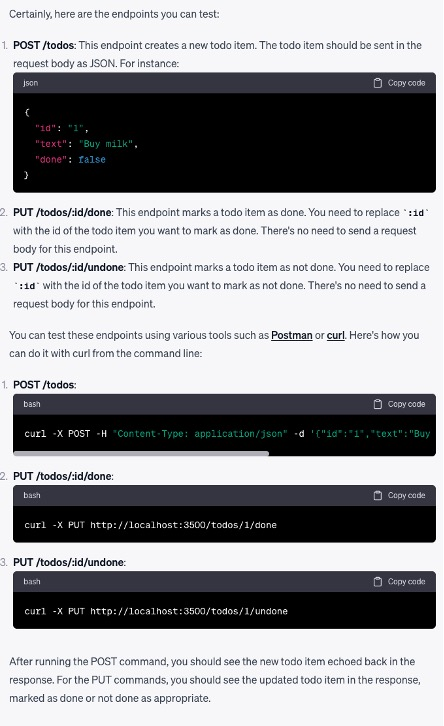
\includegraphics[width=0.5\textwidth]{Pictures/Picture25.jpg}
    \caption{Description of Picture25}
    \label{fig:picture25}
\end{figure}
\begin{figure}[h]
    \centering
    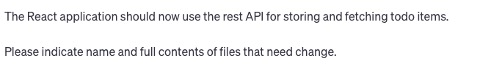
\includegraphics[width=0.5\textwidth]{Pictures/Picture26.jpg}
    \caption{Description of Picture26}
    \label{fig:picture26}
\end{figure}
\begin{figure}[h]
    \centering
    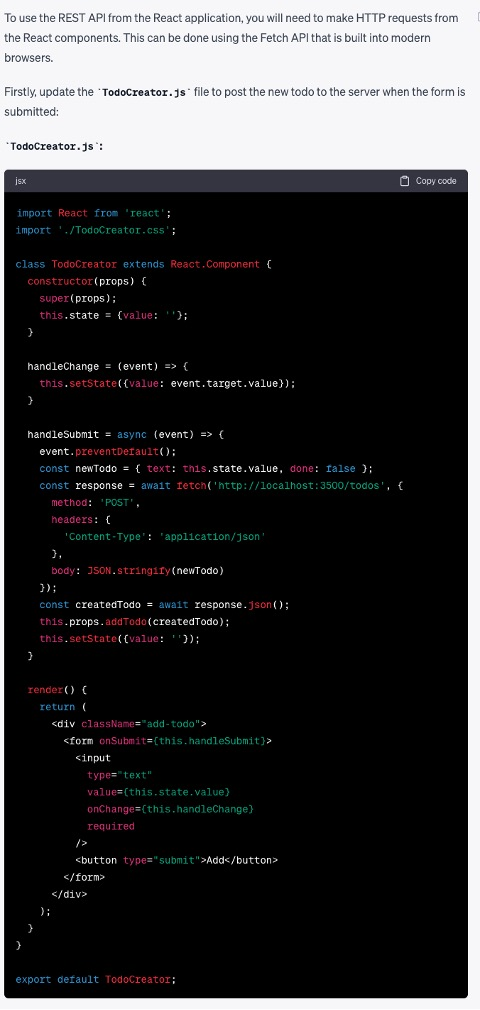
\includegraphics[width=0.5\textwidth]{Pictures/Picture27.jpg}
    \caption{Description of Picture27}
    \label{fig:picture27}
\end{figure}
\begin{figure}[h]
    \centering
    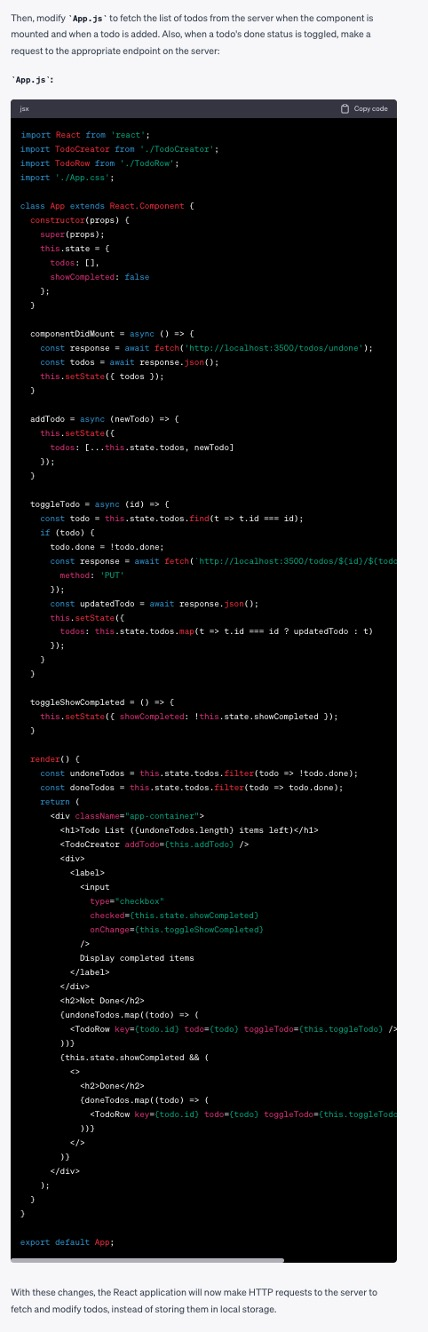
\includegraphics[width=0.5\textwidth]{Pictures/Picture28.jpg}
    \caption{Description of Picture28}
    \label{fig:picture28}
\end{figure}
\begin{figure}[h]
    \centering
    
\includegraphics[width=0.5\textwidth]{Pictures/Picture29.jpg}
    \caption{Description of Picture29}
    \label{fig:picture29}
\end{figure}
\begin{figure}[h]
    \centering
    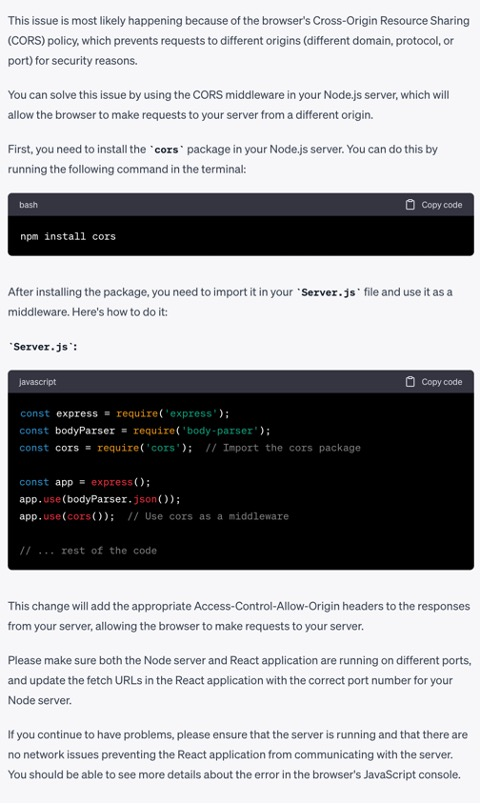
\includegraphics[width=0.5\textwidth]{Pictures/Picture30.jpg}
    \caption{Description of Picture30}
    \label{fig:picture30}
\end{figure}
\begin{figure}[h]
    \centering
    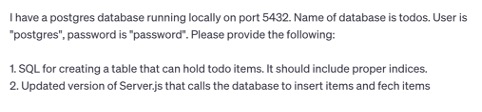
\includegraphics[width=0.5\textwidth]{Pictures/Picture31.jpg}
    \caption{Description of Picture31}
    \label{fig:picture31}
\end{figure}
\begin{figure}[h]
    \centering
    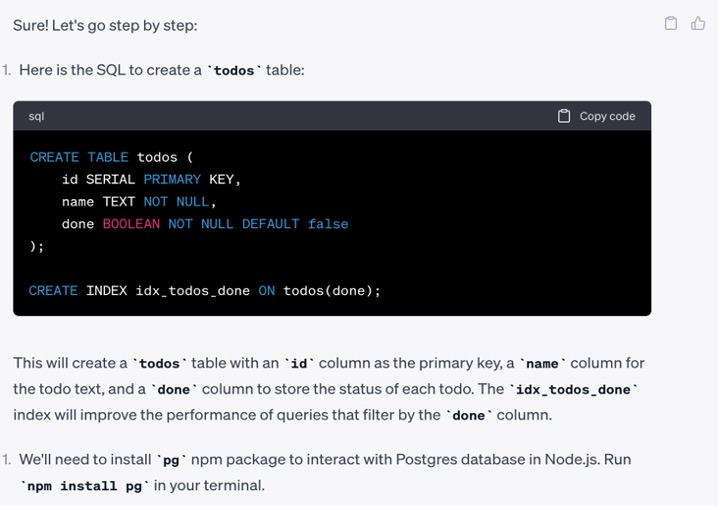
\includegraphics[width=0.5\textwidth]{Pictures/Picture31a.jpg}
    \caption{Description of Picture31a}
    \label{fig:picture31a}
\end{figure}
\begin{figure}[h]
    \centering
    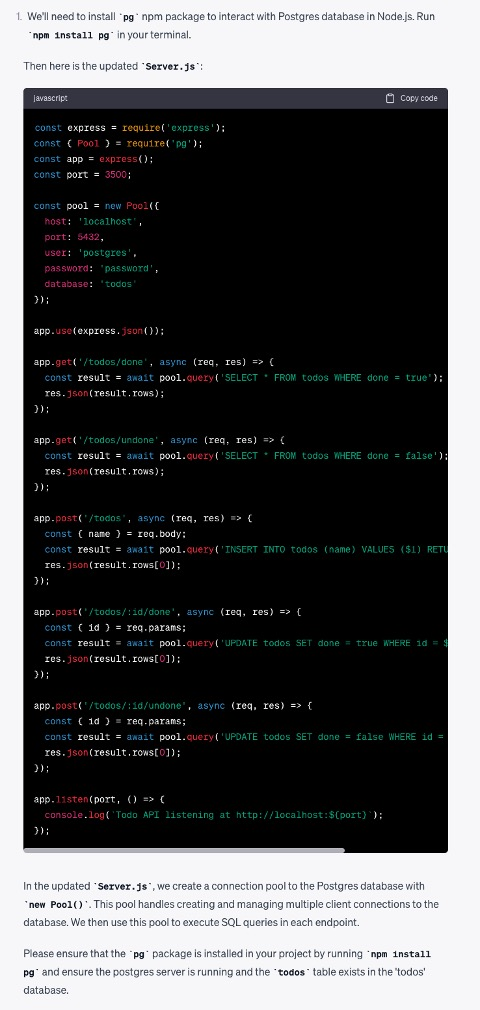
\includegraphics[width=0.5\textwidth]{Pictures/Picture32.jpg}
    \caption{Description of Picture32}
    \label{fig:picture32}
\end{figure}
\begin{figure}[h]
    \centering
    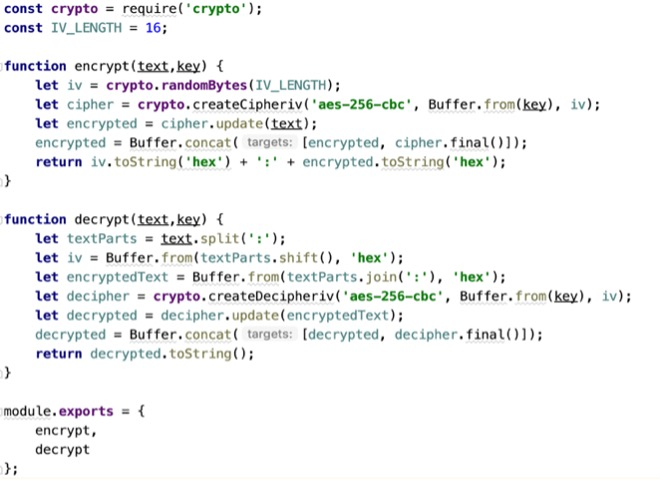
\includegraphics[width=0.5\textwidth]{Pictures/Picture33.jpg}
    \caption{Description of Picture33}
    \label{fig:picture33}
\end{figure}
\begin{figure}[h]
    \centering
    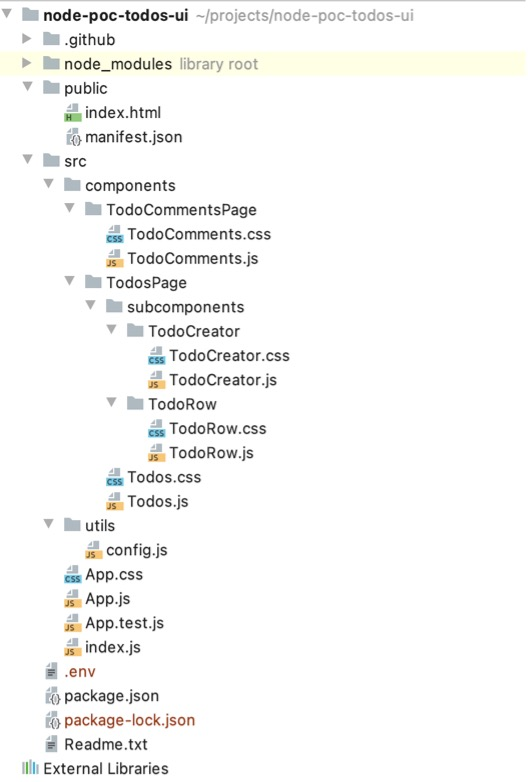
\includegraphics[width=0.5\textwidth]{Pictures/Picture34.jpg}
    \caption{Description of Picture34}
    \label{fig:picture34}
\end{figure}
\begin{figure}[h]
    \centering
    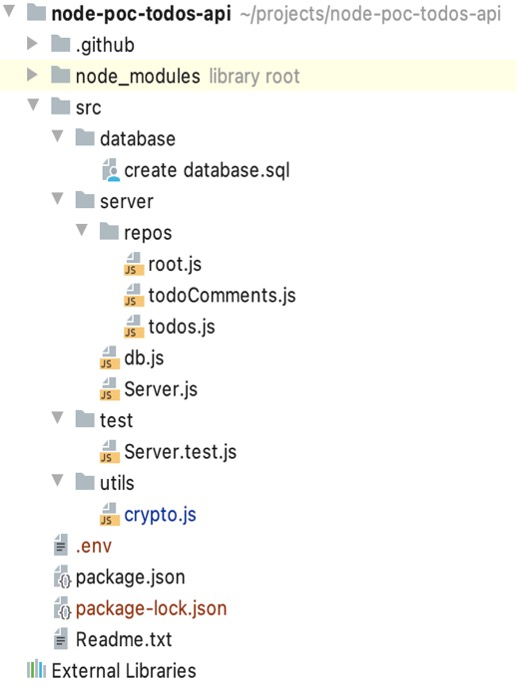
\includegraphics[width=0.5\textwidth]{Pictures/Picture35.jpg}
    \caption{Description of Picture35}
    \label{fig:picture35}
\end{figure}
\begin{figure}[h]
    \centering
    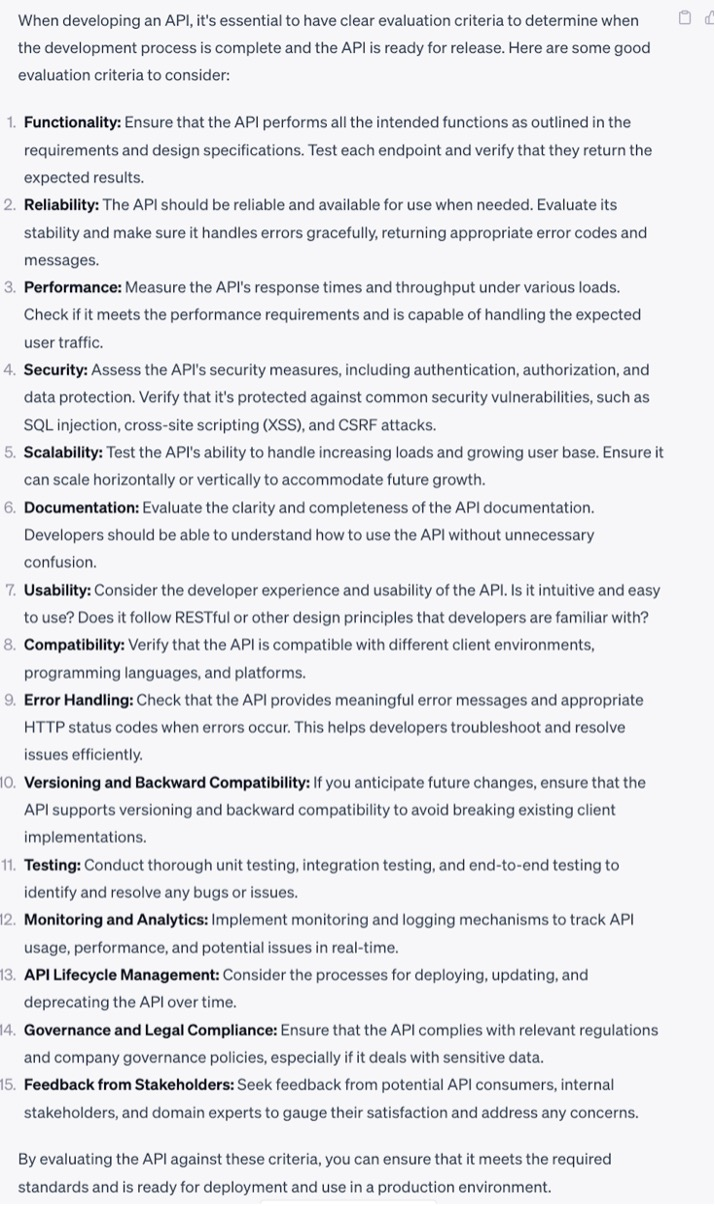
\includegraphics[width=0.5\textwidth]{Pictures/Picture36.jpg}
    \caption{Description of Picture36}
    \label{fig:picture36}
\end{figure}
\begin{figure}[h]
    \centering
    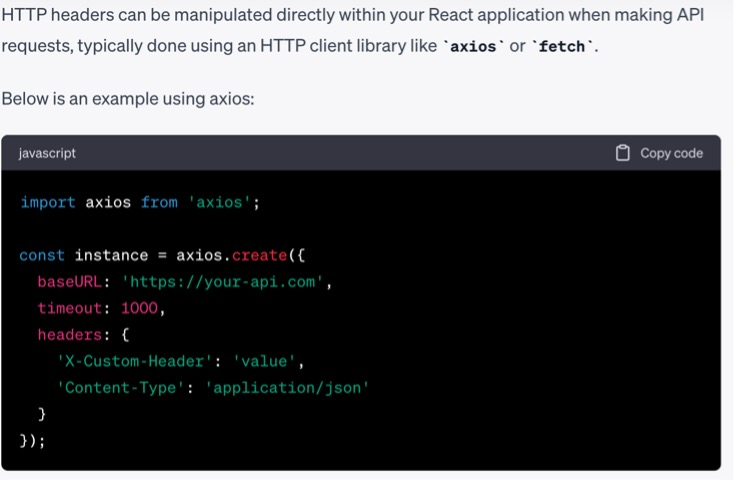
\includegraphics[width=0.5\textwidth]{Pictures/Picture37.jpg}
    \caption{Description of Picture37}
    \label{fig:picture37}
\end{figure}
\begin{figure}[h]
    \centering
    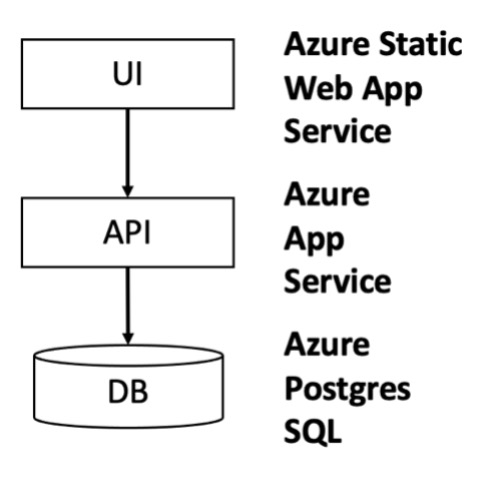
\includegraphics[width=0.5\textwidth]{Pictures/Picture38.jpg}
    \caption{Description of Picture38}
    \label{fig:picture38}
\end{figure}
\begin{figure}[h]
    \centering
    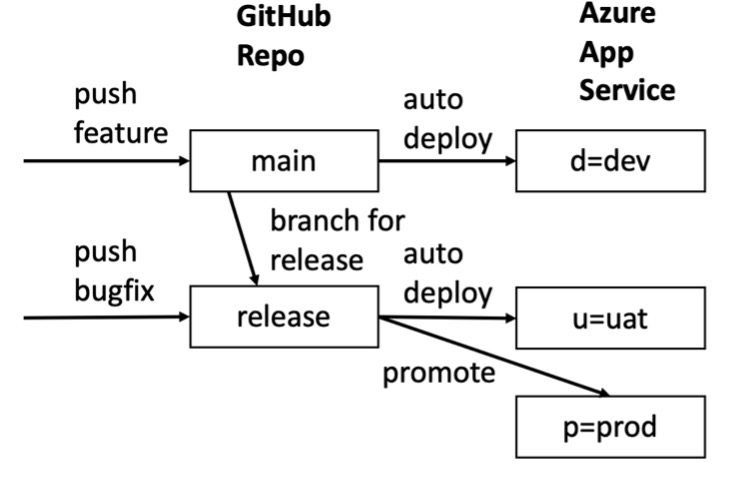
\includegraphics[width=0.5\textwidth]{Pictures/Picture39.jpg}
    \caption{Description of Picture39}
    \label{fig:picture39}
\end{figure}

\bibliography{references}
\bibliographystyle{plain} 
\end{document}

- Python example
- Transactions validation MS Powershell
- Peptide identification in Python
- ECAI tutorial

